\documentclass{report}
\usepackage{graphicx}
\usepackage{hyperref}
\title{Performance Evaluation\\Homework 1}
\author{Mahyar Emami, Rishabp Iyer}


\begin{document}

\maketitle

\section{Assignment}

In this assignment, we try to analyze and then optimize Joe's online shop 
performance, by finding the right number of access points $AP$ and servers $S$
depedning on the load of the shop (i.e., number of requests per second) denoted
by $C$.

There are 4 distict parameters that are affected by the choise of $AP$, $S$, and
$C$. These are:
\begin{itemize}
    \item $\theta$: Number of downloaded request per second (i.e., 
    throughput)
    \item $pps$: Number of packets per second over LAN.
    \item $cps$: Collision probability over LAN.
    \item $d$: delay of a request (i.e., latency).
\end{itemize}

We use a simulator to estimate these four performance metrics. The simulator
has web interface at \texttt{https://tcpip.epfl.ch/input.php}. Since we 
wanted to evaluate many design points (i.e, choice of $AP$, $S$, and $C$),
manually filling out the simulation form would be unreasonably slow. 
You can find a python function 
\texttt{runSimulation(clients, servers, apoints, sciper))} in 
\texttt{\$\{HOMEWORK\_DIRECTORY\}/scritps/remote\_simulation.py} 
that can launch the simulation given a choice of parameters and returns the
the results in a dictionary. For each subsequent section, there is a
corresponding python function that runs the simulation and stores the results
in a json file that we then used to plot the performnace metrics. Furthermore,
all the plotting utilities are in 
\texttt{\$\{HOMEWORK\_DIRECTORY\}/scritps/plotter.py} 

\subsection{Variability of the metrics}

We have used the function \texttt{PartOne} to obtain the data that is
represened in Figure~\ref{fig:part_one}. We have varied $C$, $AP$, and $S$
from 1 to 4 and obtained 64 unique input configurations. For each input 
configuration we have run the simulation 10 times to observer the variability 
of performnace metrics. Evidently, there can be a lot of veriabilty at each 
point.
\begin{figure}[h]
    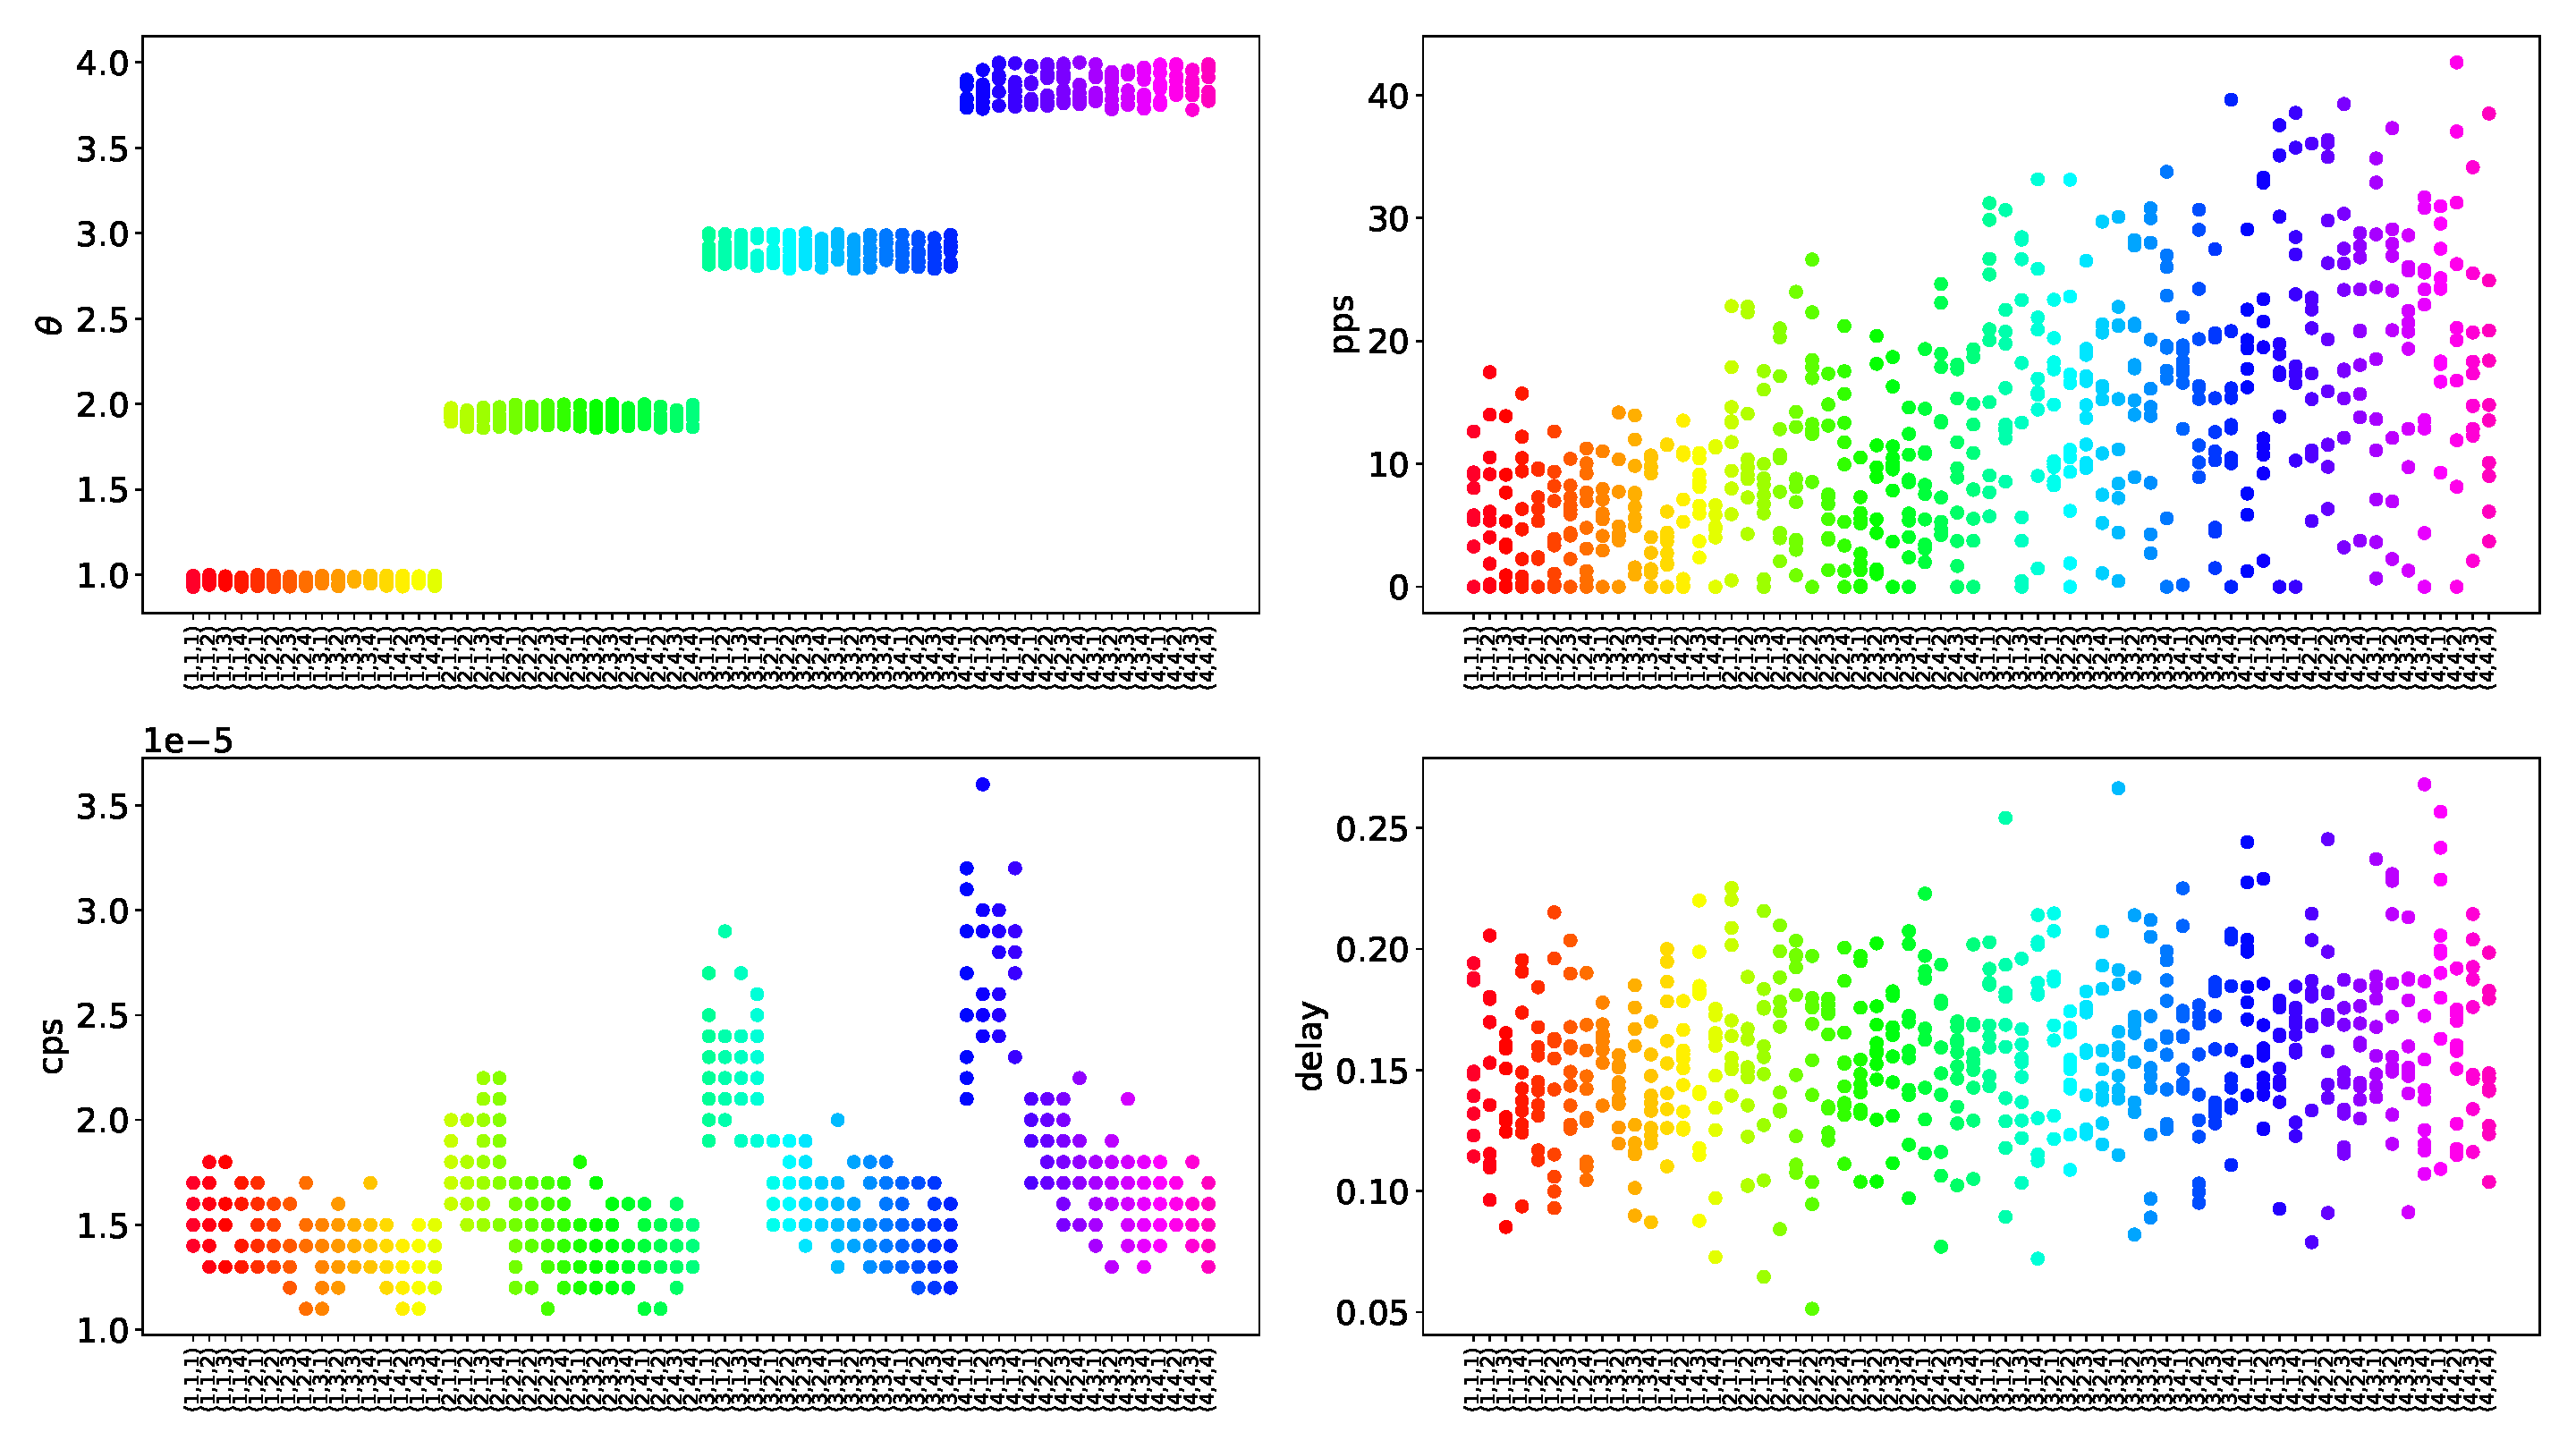
\includegraphics[width=\linewidth]{/home/mayy/courses/PE/COM-503/homework-1/data/part_one.pdf}
    \label{fig:part_one}
    \caption{Variability of throughput, packets per second, collision 
    probability and delay for various input parameters. Each point on the 
    horizontal axis corresponds to a tuple ($C, APS, S$). Points on the 
    vertical axis have the same color and correspond to 10 repeated experiments
    using the values in the tuple on the horizontal axis. Different colors 
    denote different input configurations.}
\end{figure}


\subsection{Using minimum resources, $AP=S=1$}

Not surprisingly, Joe wants to keep the cost of his operattion minimal.
He would like to know the maximum load he can sustain with a single server
and a single access point. We start from 10 clients (i.e., $C=10$) and 
linearly increase the number of clients with a step of $10$ up to $1000$ and
collect the performance metrics (see function \texttt{PartTwo}). 
Figure~\ref{fig:part_two} illustrates the results of 10 repeated simulations. 
The horizontal axis is the number of requests per second (i.e., $C$) and
the error bars show the 0.1 and 0.9 quantiles.
Evidently, linear increase is throughput (i.e., $\theta$) with less than
100 requests per second and the collision probability shoots up. Packets per 
second increase slows down around the same points and delay starts to increse
super-linearly. This shows that the system is bottlenecked and can not 
sustain a linear increase in throughput with a linear increase in the load.



\begin{figure}[h]
    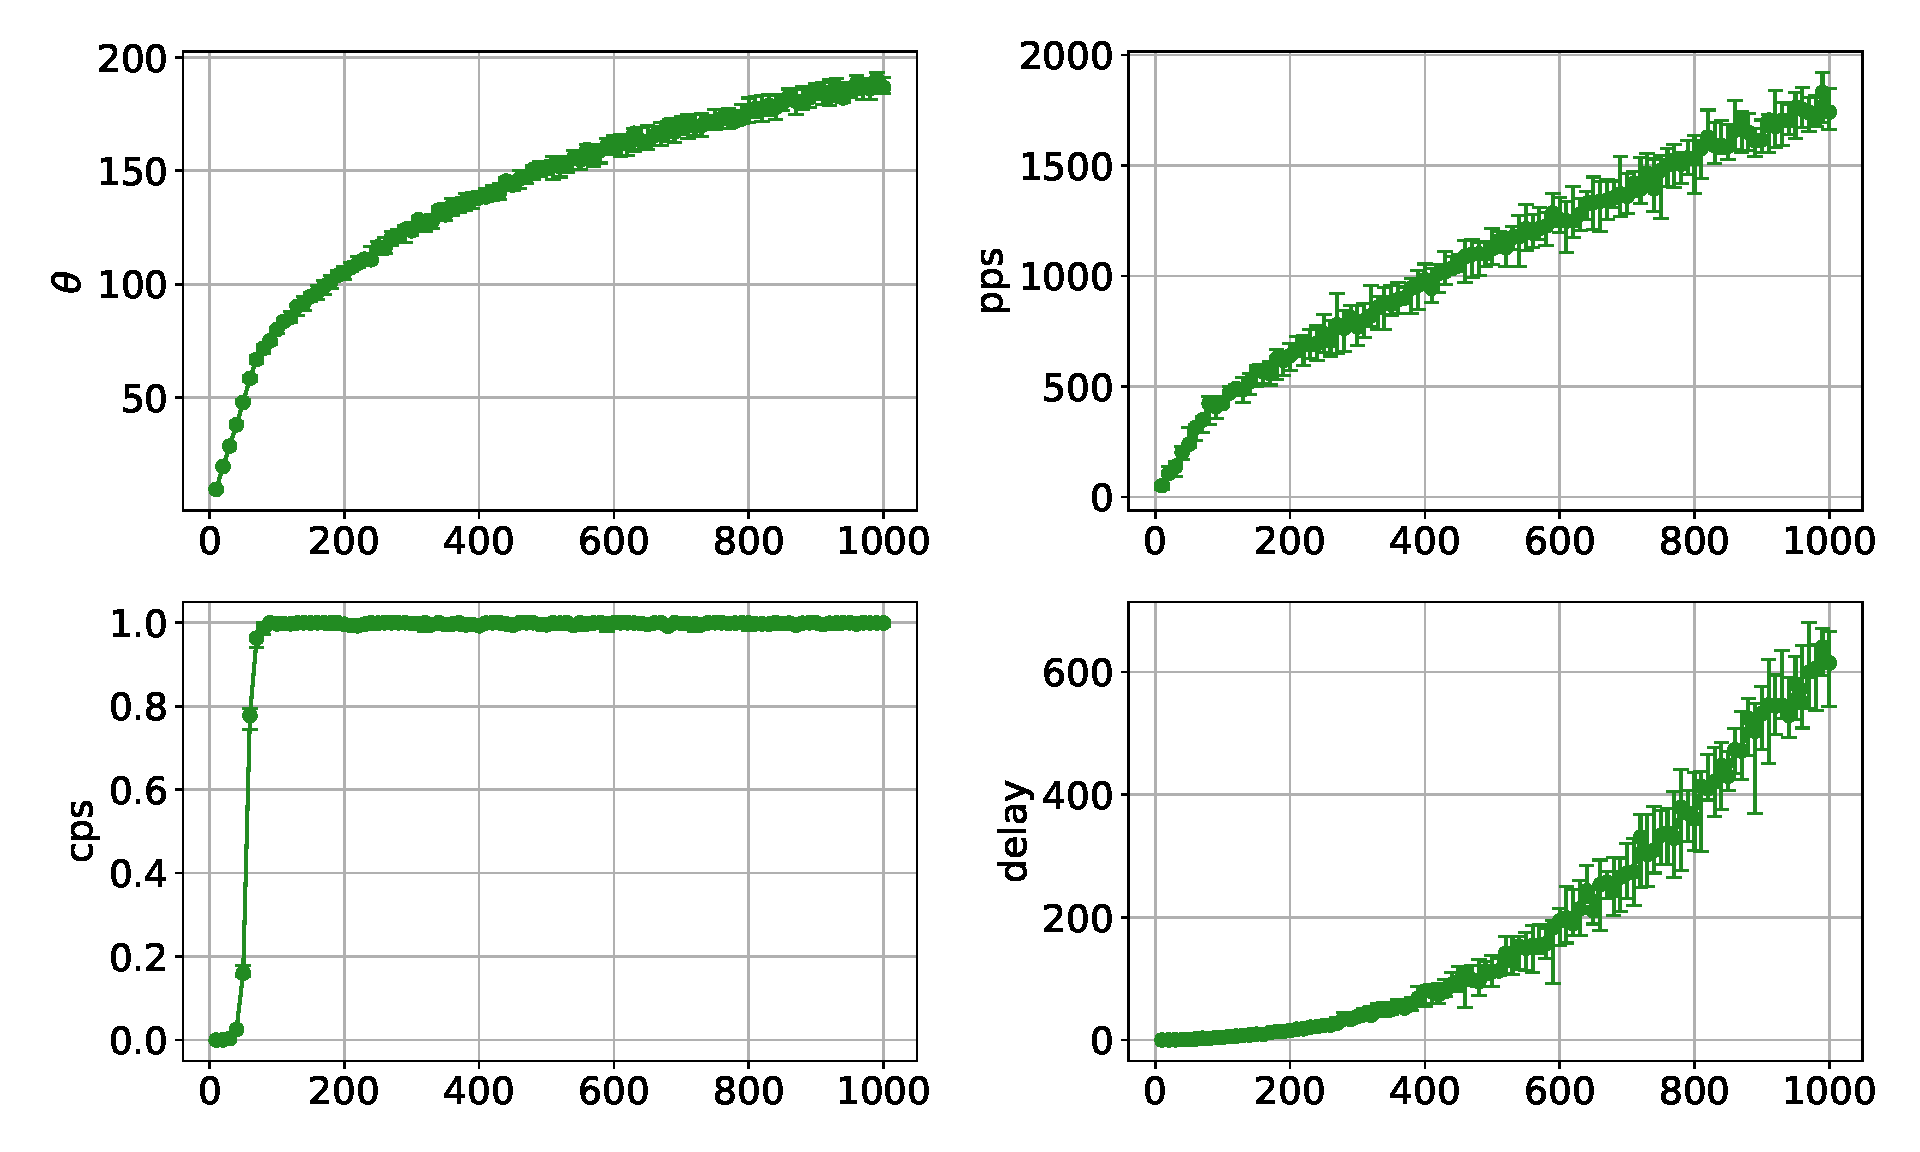
\includegraphics[width=\linewidth]{../data/part_two.pdf}
    \label{fig:part_two}
    \caption{Performance metrics of Joe's shop with having a single access
    point and a single server. Throuhgput subsides with increased request per
    second and delay rises superlinearly. Collision probability shoots 
    up to a ceiling while packets per second follows the same trend as 
    throughput.}
\end{figure}

\subsection{More access points}
When we showed Figure~\ref{fig:part_two} to a bystander at Flon metro station, 
they immediately suggested that we should double the number of access points.
Their rational was that with more access points, more traffic can reach the
servers the throughput should linearly increase up to a larger number of 
requests per second. We tested this intuition by keeping $S=1$ and 
increasing increasing $AP$ up to 4. The results are summarized in 
Figure~\ref{fig:part_three}. As apparent, the shop can now sustain a higher
throughput before a sharp fall from grace. Unfortunately, the delay becomes
worse in this case. In fact, around where the delay reaches its sealing of 
1000 seconds, the throughput drops instead of becoming flat. This seems to 
be a congestion collapse that was not really visible with a single access point.
Furthermore, there is a valley in the collision probability with 4 access points
which we do not have an explanation for. The packest per second follows the
same trend as the throughtput and drops when the delay sees a sharp 
rise. This leaves us to wonder whether \emph{only increasing the access points}
is a good idea. The following sections will try to find a better solution for
Joe.

\begin{figure}[h]
    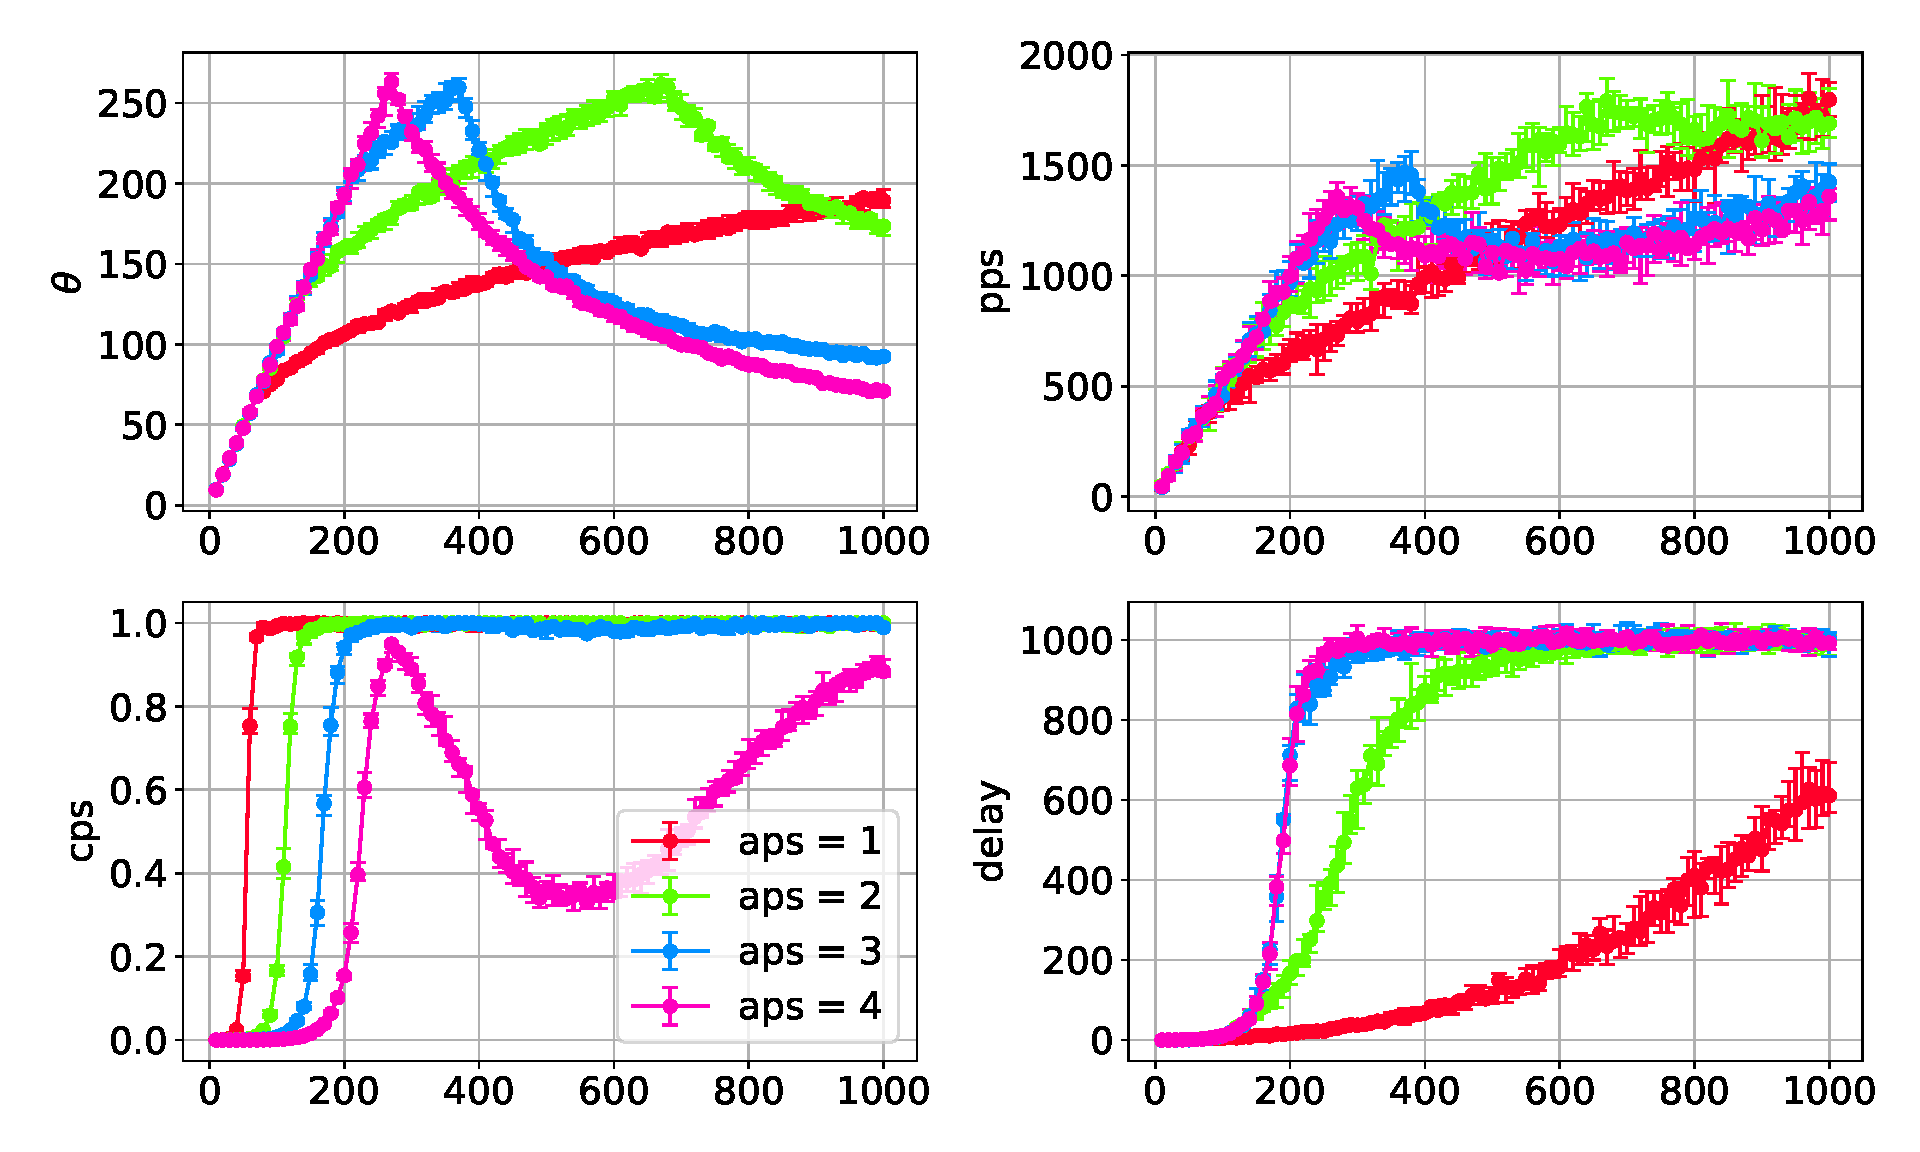
\includegraphics[width=\linewidth]{../data/part_three.pdf}
    \label{fig:part_three}
    \caption{Performance metrics with having a single server with 
    up to 4 access points. While more access points help with throghput, 
    after some point the delay reaches a ceiling and causes congestion collpase
    (for instance request could be dropped at the server).}
\end{figure}

\subsection{More servers}

Naturally, there was some other bystander who believed more in CPU power than
access point bandwidth. To be fair to everyone who have propsed a solution, 
we have also tried out keeping $APS=1$ and increasing the number of servers
to 4. Figure~\ref{fig:part_four} depicts this experiment, Sadly, increasing the
server count yields almost no tangible improvement. Only the delay is 
improved. This may suggest that there is some form of queueing at the servers
that gets evened out among multiple servers and hence the reduction in delay.

\begin{figure}[h]
    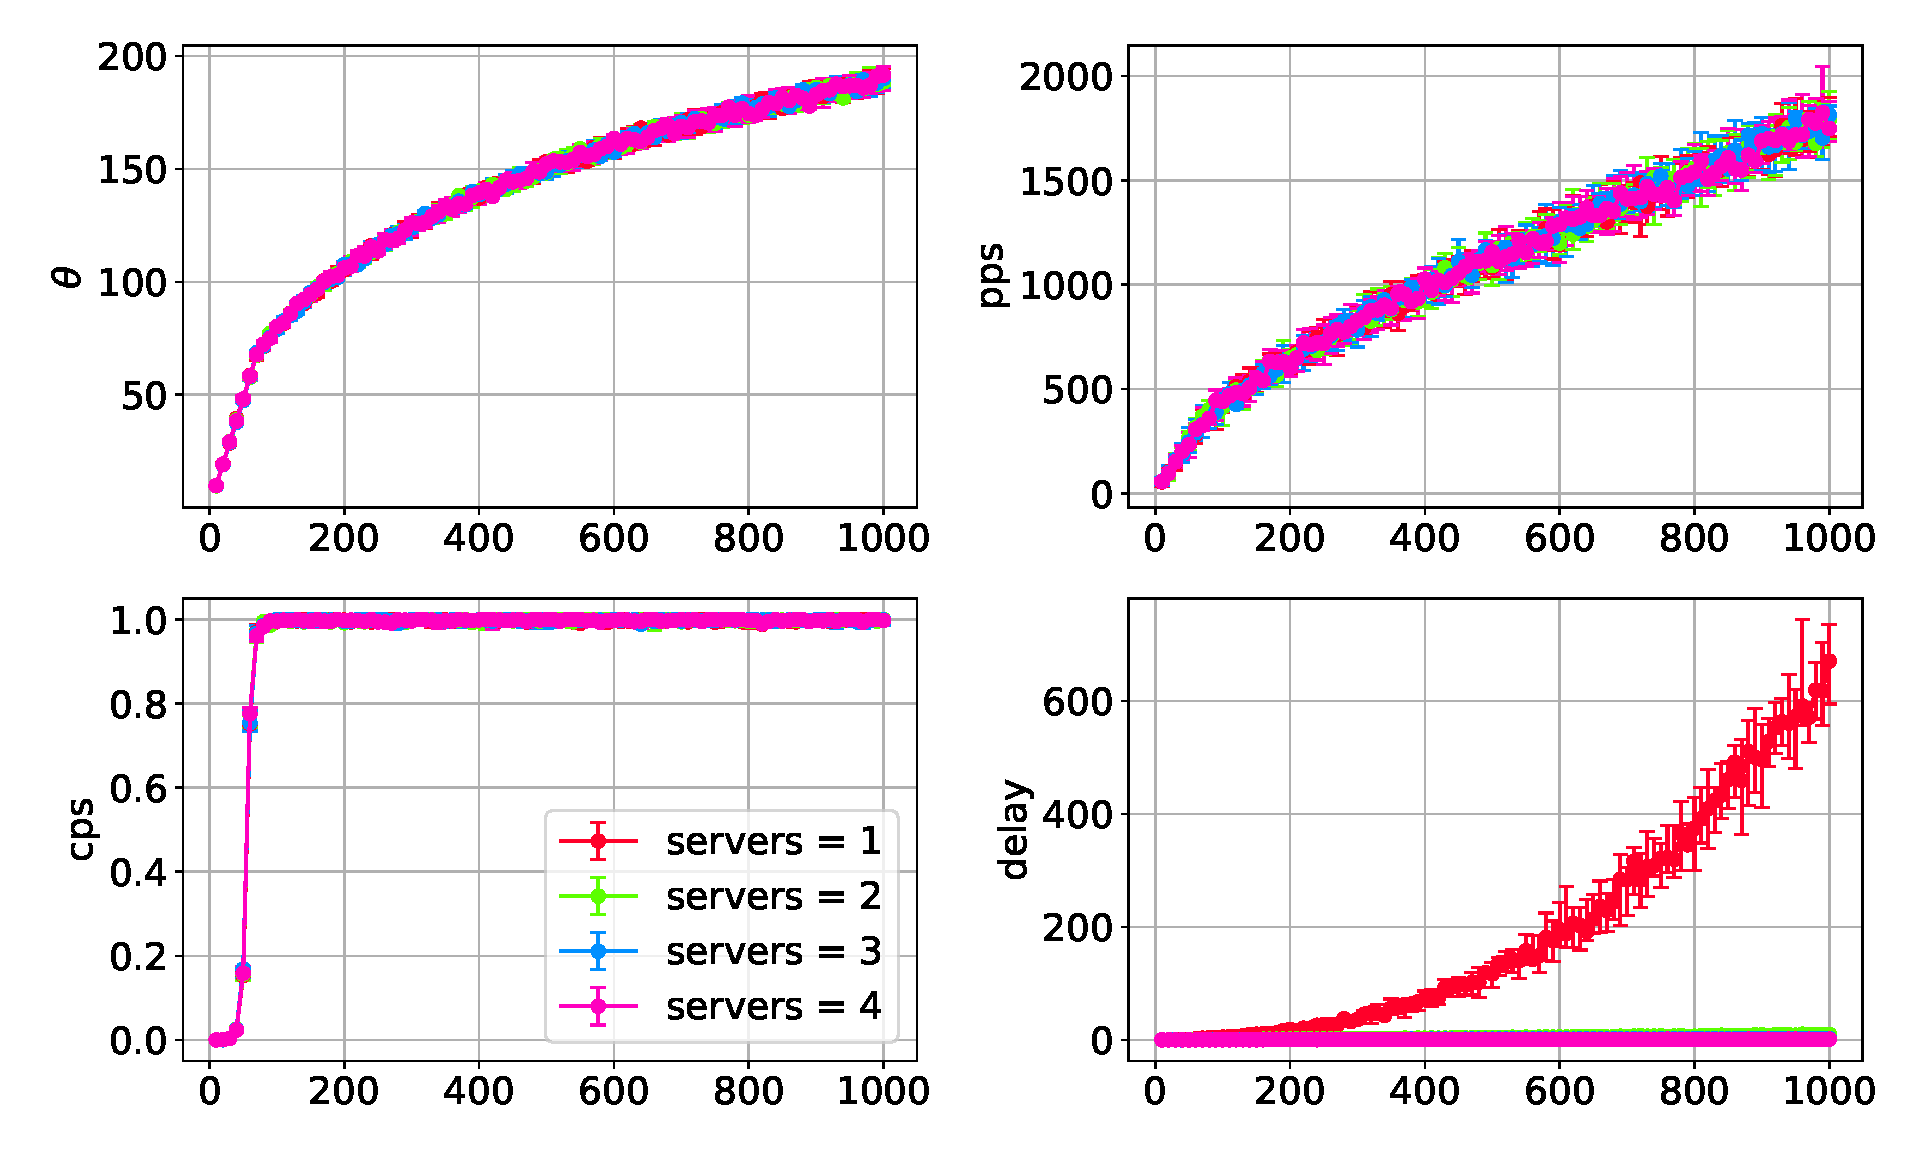
\includegraphics[width=\linewidth]{../data/part_four.pdf}
    \label{fig:part_four}
    \caption{Performnace metrics with two a single access point and
    1 to 4 servers. It seems that having more servers without extra access
    points is fruitless for thoughput and only helps with delay.}
\end{figure}

\subsection{More servers and more access point at the same time}

The previous two sections somehow revealed two trends:(i) more access points
are good for throughput, but can lead to congestion collapes, and (ii) more
servers seem to help with delay, which may be the cause of congestion collapse.

In this section, we kept the $APS=2$ and tried out having 1 to 4 servers
(i.e., same as last section but with one more access point). The 
results are showed in Figure~\ref{fig:part_five}. Clearly, the congestion
collapse observerd with one server and two access points is no longer visible 
with two servers (red curve vs. green). However, with two servers and 
and two access points, the delay can increase again which a warning for 
congestion collapse.

\begin{figure}[h]
    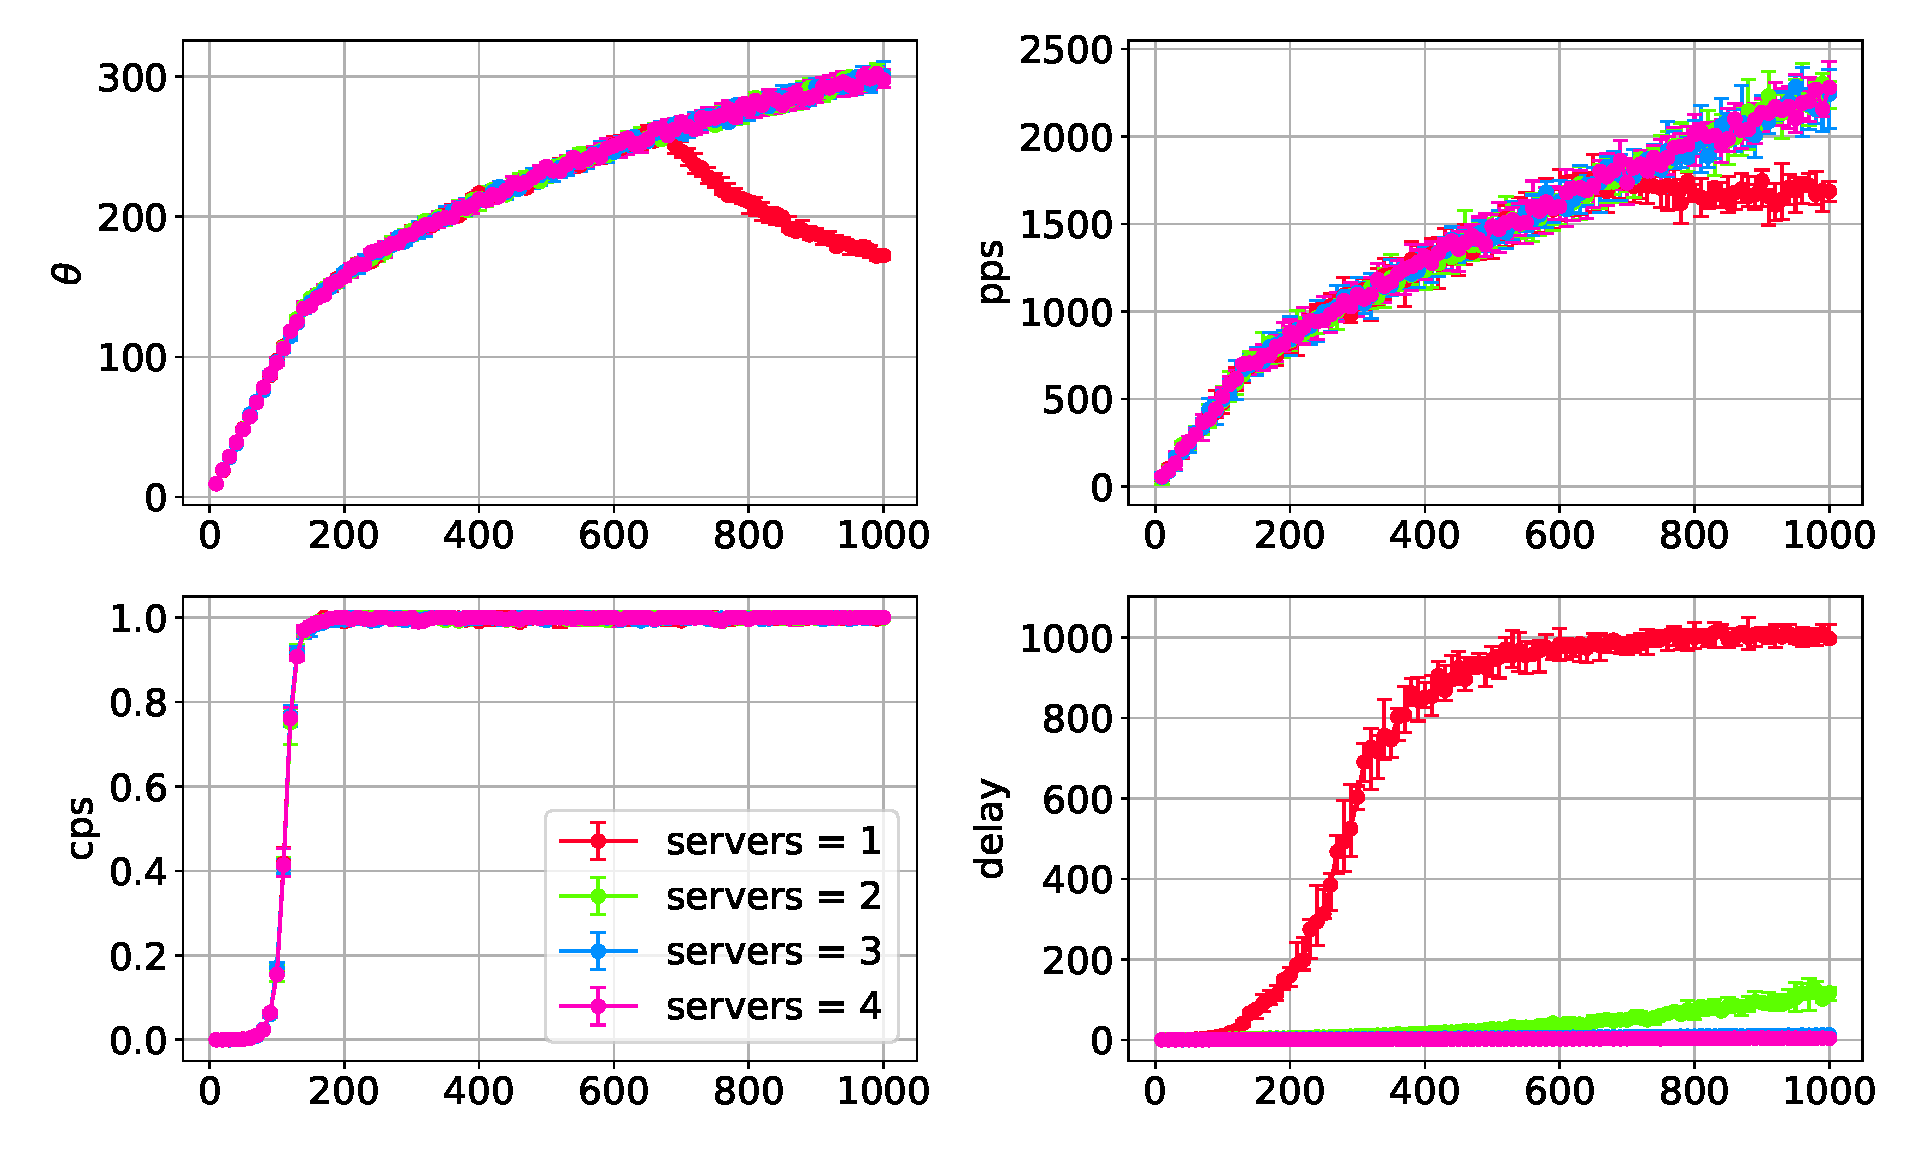
\includegraphics[width=\linewidth]{../data/part_five.pdf}
    \label{fig:part_five}
    \caption{Performance metrics with 2 access point and 1 to 4 
    servers. Evidently, congestion collapse can be avoided with more 
    servers.}
\end{figure}

Interestingly, the delay with with two servers sees a sharper increase when 
there are 3 access points compared to 2.


So far, we can conclude that access points are necessary for throughput, but
with few servers, delay shoots up and congestion collapse causes throughput 
drops. To derive a final rule of thumb, we use the maximum number of 
$APS = 10$ and increase the servers from 1 to 10 to find the bounds of 
throughput and congetstion collapse. 
Figure~\ref{fig:part_seven} outlines this experiment. This clearly demostrates
that having more than 4 severs has no throughput benefit as in the worse case
of having 10 access points and 1000 requests per second, congestion collapse
nearly \emph{starts} to happen with 4 servers.

\begin{figure}[h]
    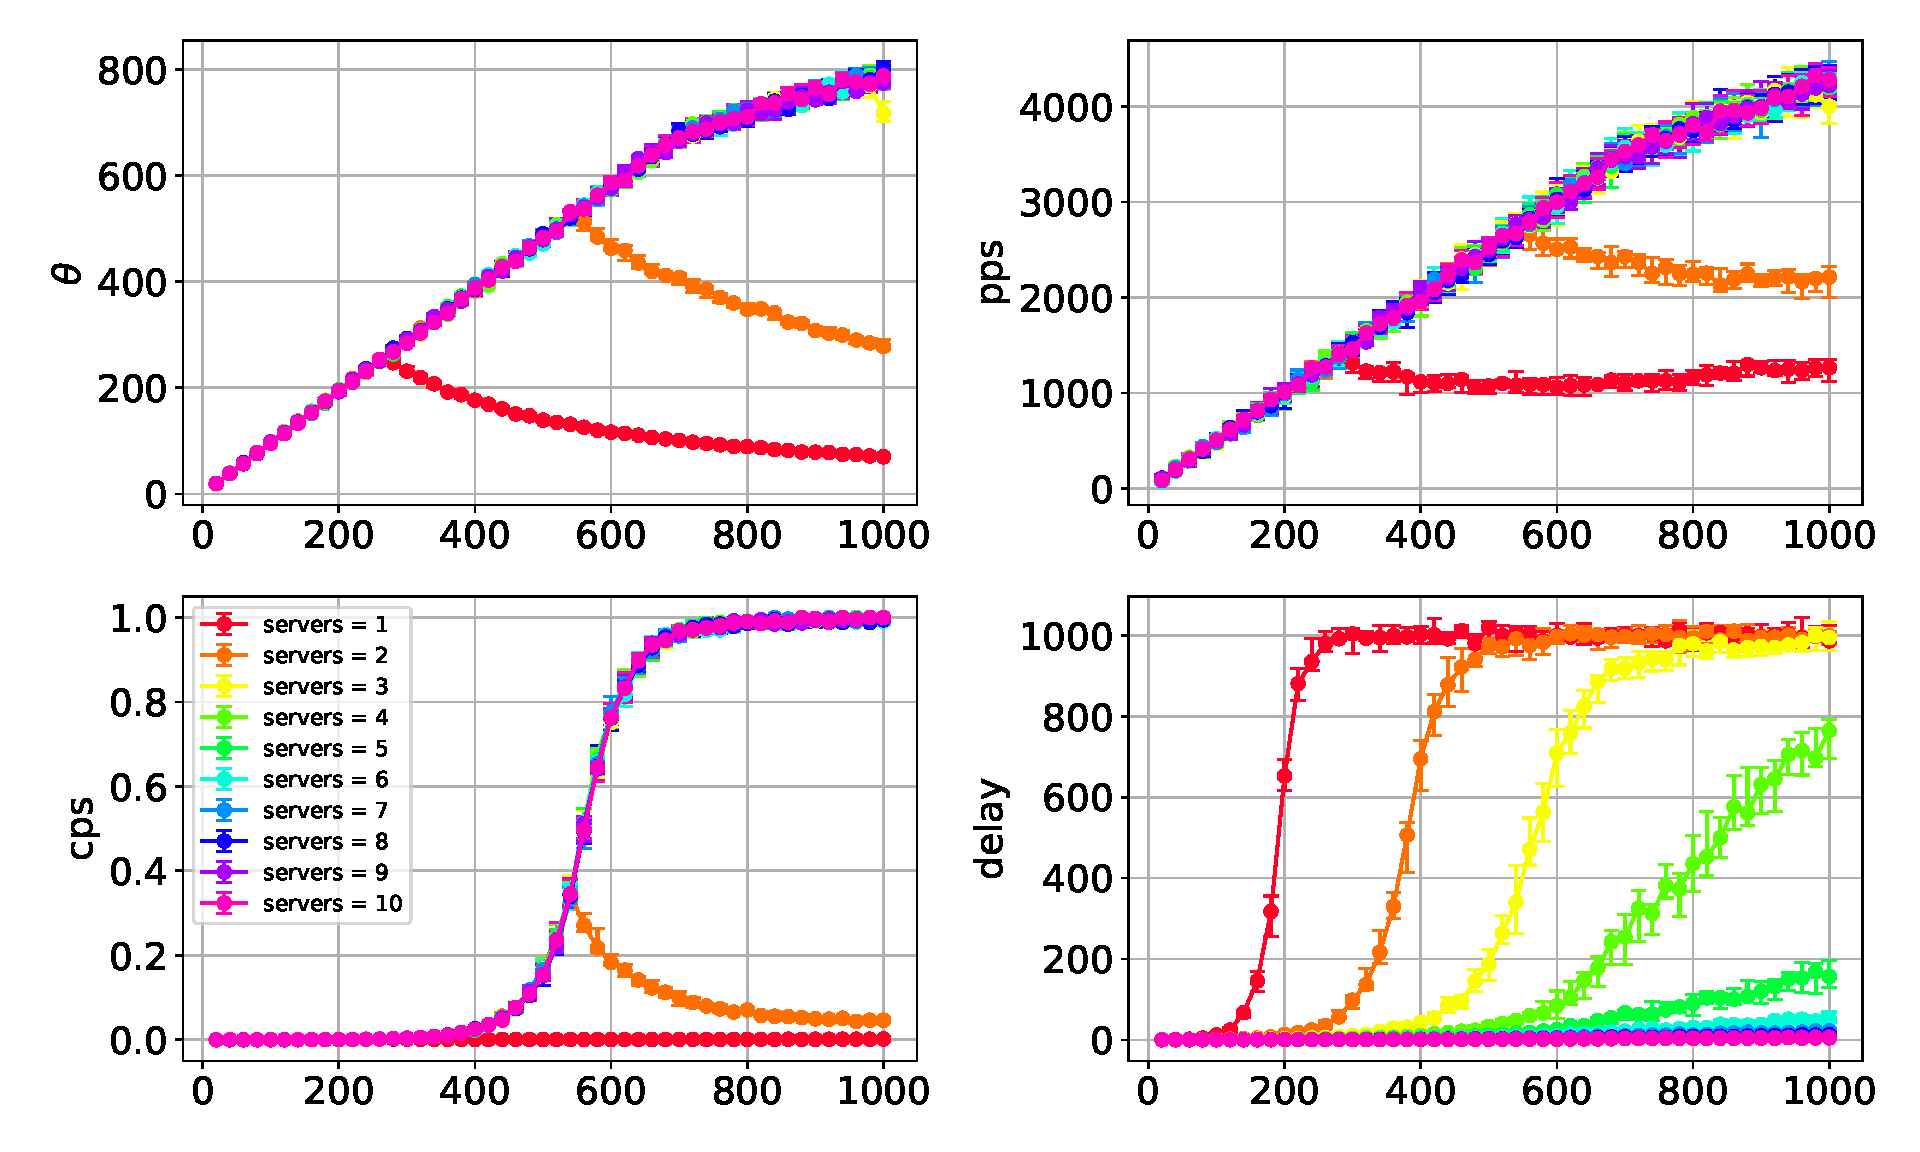
\includegraphics[width=\linewidth]{../data/part_seven.pdf}
    \label{fig:part_seven}
    \caption{Performance metrics with maximum number of 10 access points 
    (maximum) and 1 to 10 servers. More than 4 servers has no practical 
    benefits as congestion collapse with not happen even at maximum load.}
\end{figure}

Finally, by keeping the number of servers to 4 we tried out having 1 to 10 
access points to identify where throughput increase experiences a \emph{knee}.
Figure~\ref{fig:part_eight} delineates the outcome of this experiment. Clearly,
the knee happens at some point, and clearly the increasing the number of servers
would not avoid that as Figure~\ref{fig:part_seven} showed before. However,
depending on the anticipated load, Joe's can now pick the right number of access
points and then the servers. Intuitively, we can have
$APS = \floor{C_{max} / 100}$ and where $C_{max}$ is the maximum anticipated 
load. And then $S = min\{4, \ceil{APS / 2}\}$. Although the second rule
is somewhat conservative and in a specific case fewer servers can be used.


\begin{figure}[h]
    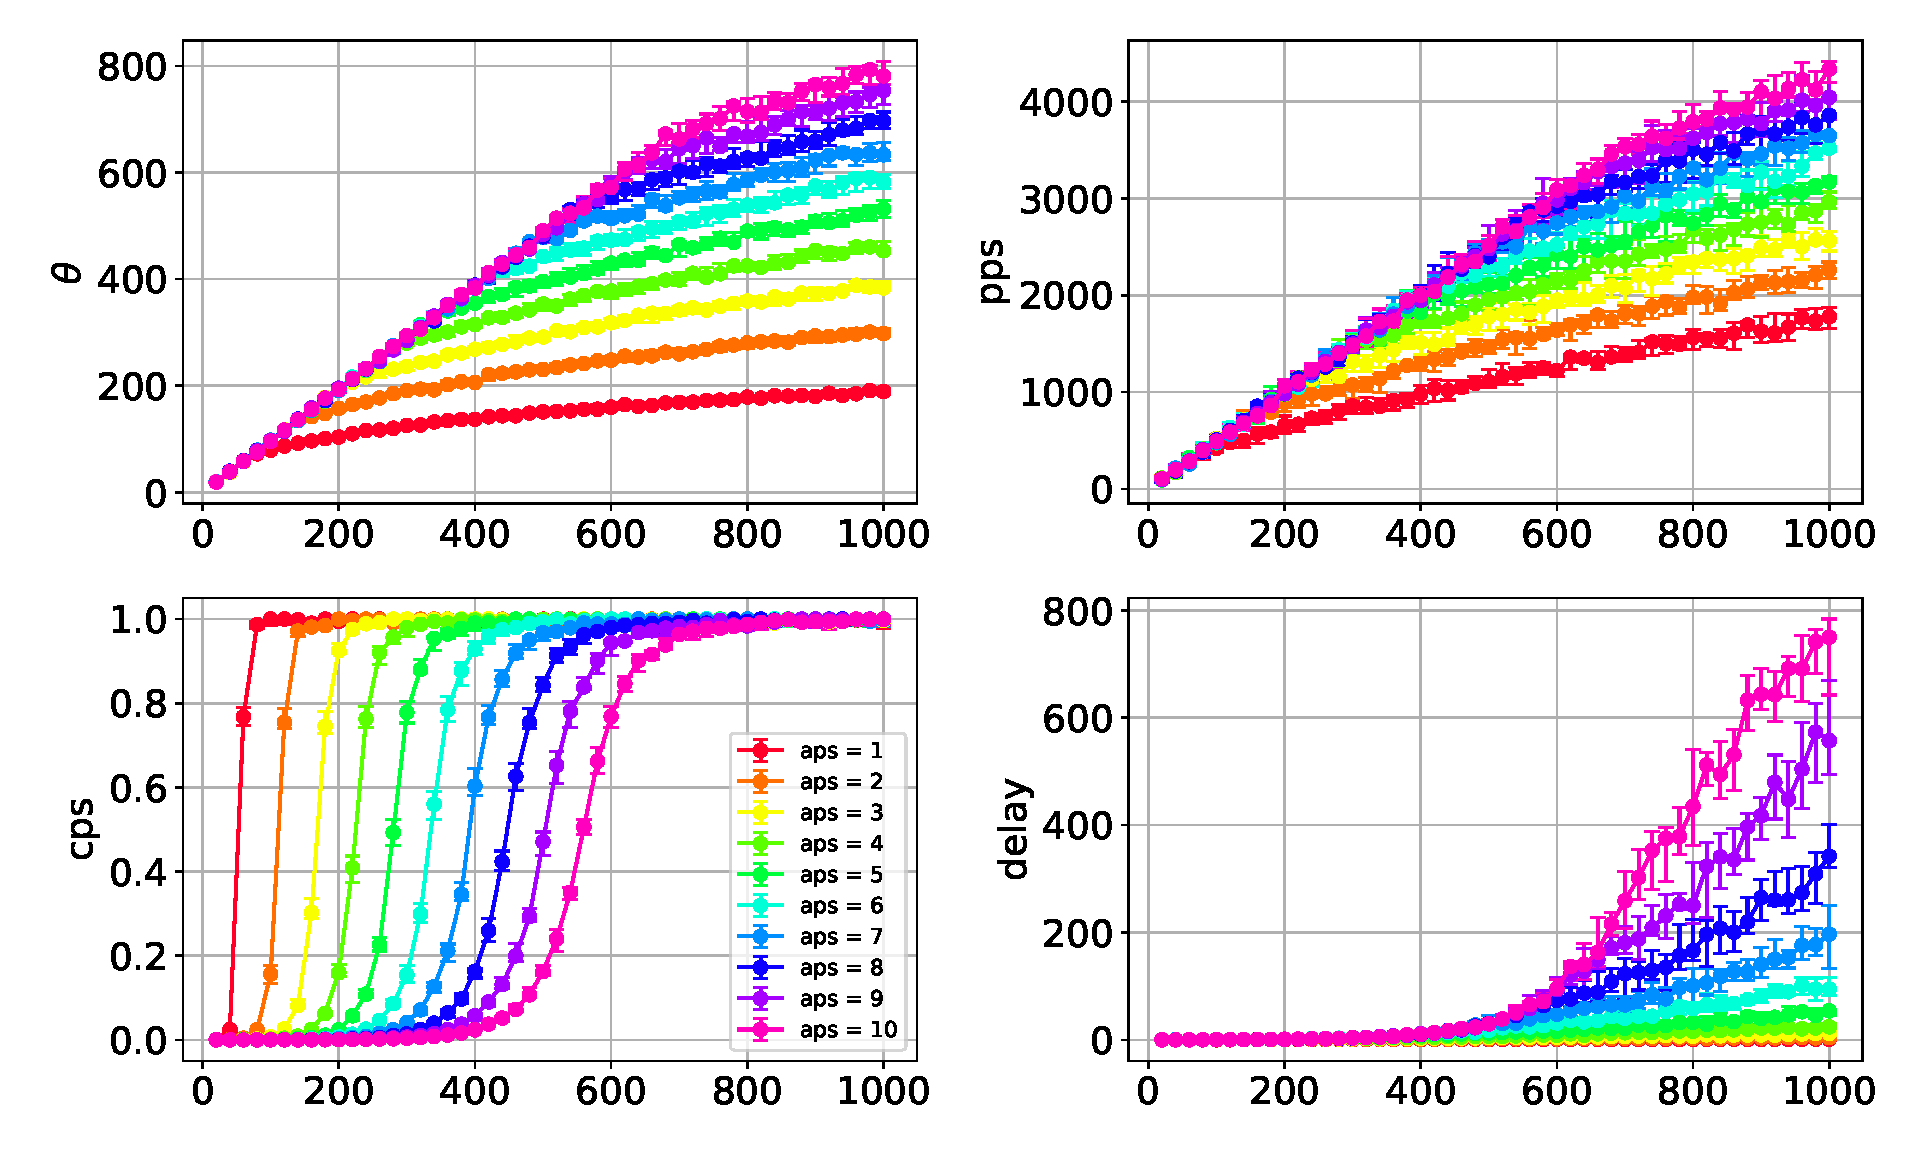
\includegraphics[width=\linewidth]{../data/part_eight.pdf}
    \label{fig:part_eight}
    \caption{Performance metrics with having 4 servers and 1 to 10 access points.
    Understandably, throughput knee can be shifted towards the right with 
    more access points. Furthermore, with 4 servers congestion collapse is
    entirely avoided as the delay remains below the ceiling.}
\end{figure}



\end{document}